\documentclass[12pt]{article}
\usepackage[utf8]{inputenc}
\usepackage{graphics}
\usepackage{graphicx}
\usepackage{float}
\usepackage{hyperref}
\hypersetup{
	colorlinks=true,
	linkcolor=blue,
	filecolor=magenta,      
	urlcolor=cyan,
}

\title{Het softwarewijzigingsproces vastleggen}
\author{Thomas van Dongen, Koen Schilders}
\date{14 maart 2018}

\begin{document}


% De titelpagina
\begin{titlepage}
\maketitle
\end{titlepage}


\section{Doelstelling}
In dit document wordt een softwarewijzigingsproces beschreven waardoor de software in productie op een effectieve manier kan worden onderhouden. Een softwarewijzigingsproces maakt duidelijk welke taken bij elke betrokken rol hoort.
% TODO: SMART-manier van het doel van dit proces beschrijven, gericht op ESD6


\section{Het softwarewijzigingsproces}
\subsection{Rollen}
% TODO: Benoem de rollen en omschrijf deze
% TODO: Per rol beschrijven welke verantwoordelijkheden
\subsubsection{Gebruiker/Klant}
Lorem ipsum dolor sit amet.

\medskip
\noindent\textbf{Verantwoordelijkheden:}
\begin{itemize}
	\item Verantwoordelijkheid 1
\end{itemize}

\subsubsection{Tester}
Lorem ipsum dolor sit amet.

\medskip
\noindent\textbf{Verantwoordelijkheden:}
\begin{itemize}
	\item Verantwoordelijkheid 1
\end{itemize}

\subsubsection{Ontwikkelaar}
Lorem ipsum dolor sit amet.

\medskip
\noindent\textbf{Verantwoordelijkheden:}
\begin{itemize}
	\item Verantwoordelijkheid 1
\end{itemize}

\subsubsection{Productowner}
Lorem ipsum dolor sit amet.

\medskip
\noindent\textbf{Verantwoordelijkheden:}
\begin{itemize}
	\item Verantwoordelijkheid 1
\end{itemize}



\subsection{UML-Activity diagram}
%\begin{figure}[H]
%	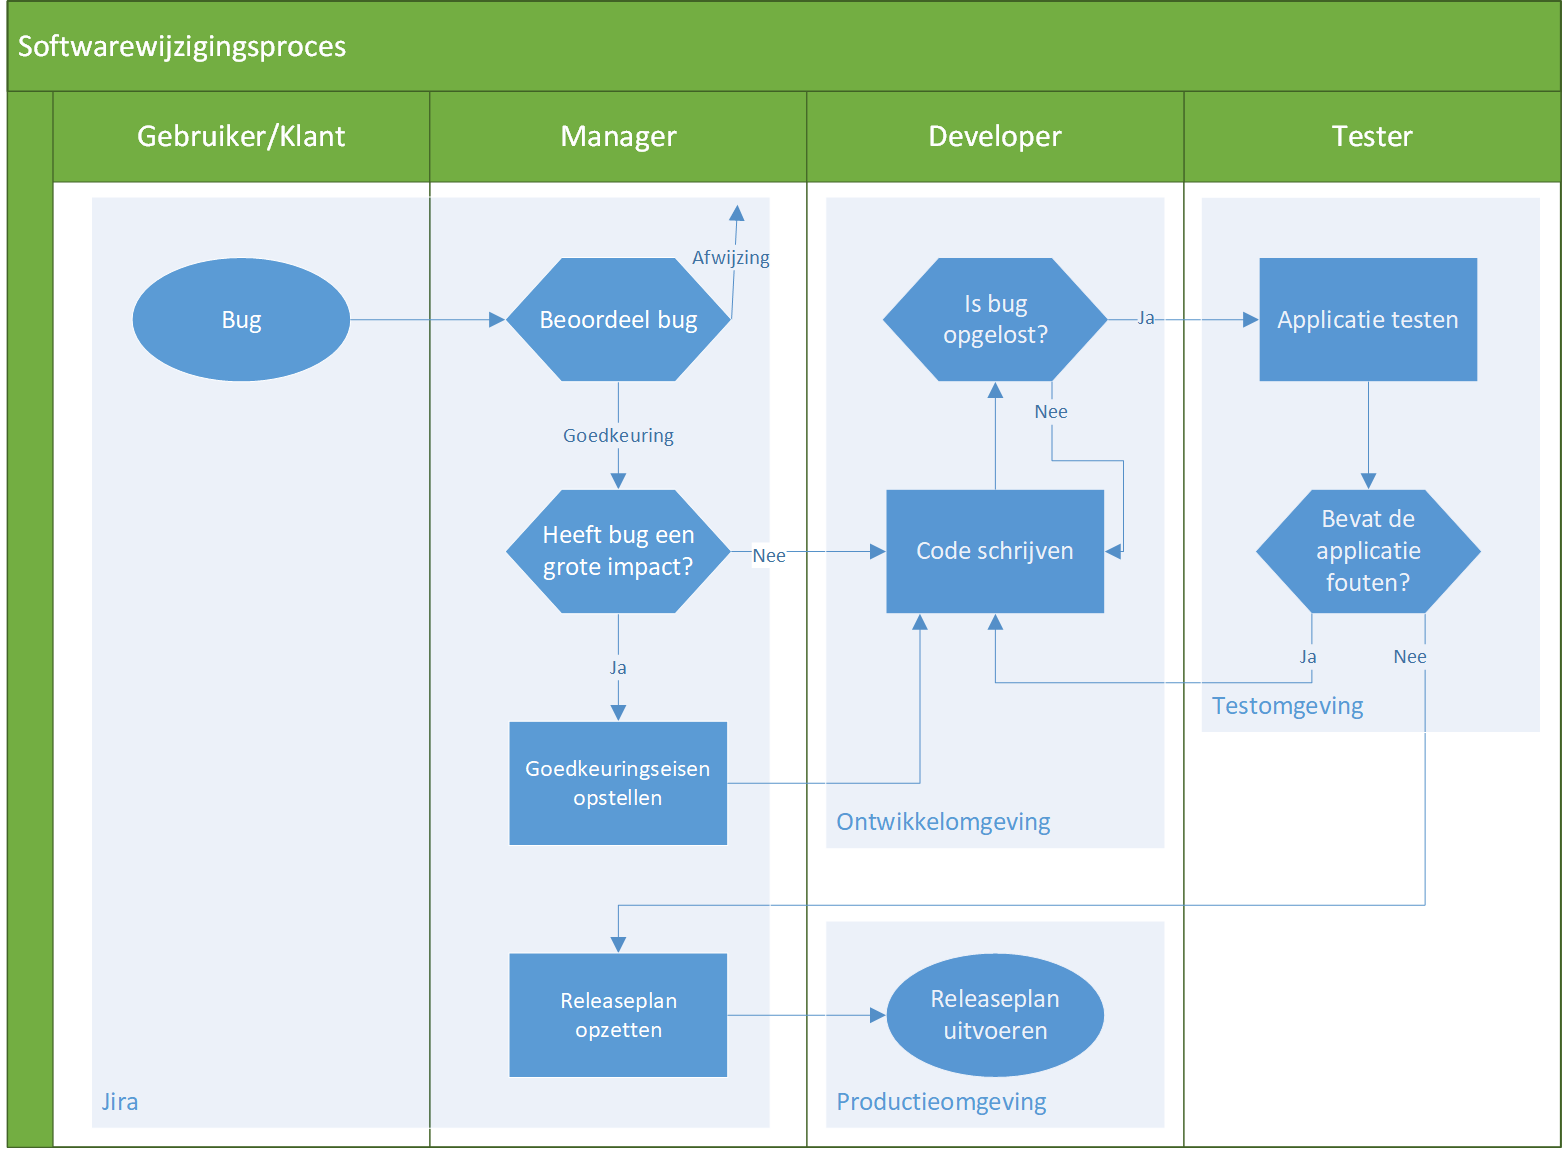
\includegraphics[width=\textwidth]{images/UMLActivityDiagram.png}
%	\caption{Diagram van het softwarewijzigingsproces.}
%\end{figure}

% UML-Activity diagram maken, incl swimlanes voor verschillende rollen
% Diagram beschrijven, uitleg over ontwerpkeuzes
% Diagram moet duidelijk maken wie welke taak uitvoert, met welke tooling en welke (OTAP) omgeving


% Werkinstructies voor wat ingewikkeldere taken in het diagram


% Sources
\begin{thebibliography}{9}
	\bibitem{shortcode_name}
	Name of author,
	\textit{Title of page or book},
	Date of publication,
	\url{https://google.com}
\end{thebibliography}

\end{document}